% Options for packages loaded elsewhere
\PassOptionsToPackage{unicode}{hyperref}
\PassOptionsToPackage{hyphens}{url}
%
\documentclass[
]{article}
\usepackage{amsmath,amssymb}
\usepackage{lmodern}
\usepackage{ifxetex,ifluatex}
\ifnum 0\ifxetex 1\fi\ifluatex 1\fi=0 % if pdftex
  \usepackage[T1]{fontenc}
  \usepackage[utf8]{inputenc}
  \usepackage{textcomp} % provide euro and other symbols
\else % if luatex or xetex
  \usepackage{unicode-math}
  \defaultfontfeatures{Scale=MatchLowercase}
  \defaultfontfeatures[\rmfamily]{Ligatures=TeX,Scale=1}
\fi
% Use upquote if available, for straight quotes in verbatim environments
\IfFileExists{upquote.sty}{\usepackage{upquote}}{}
\IfFileExists{microtype.sty}{% use microtype if available
  \usepackage[]{microtype}
  \UseMicrotypeSet[protrusion]{basicmath} % disable protrusion for tt fonts
}{}
\makeatletter
\@ifundefined{KOMAClassName}{% if non-KOMA class
  \IfFileExists{parskip.sty}{%
    \usepackage{parskip}
  }{% else
    \setlength{\parindent}{0pt}
    \setlength{\parskip}{6pt plus 2pt minus 1pt}}
}{% if KOMA class
  \KOMAoptions{parskip=half}}
\makeatother
\usepackage{xcolor}
\IfFileExists{xurl.sty}{\usepackage{xurl}}{} % add URL line breaks if available
\IfFileExists{bookmark.sty}{\usepackage{bookmark}}{\usepackage{hyperref}}
\hypersetup{
  pdftitle={ClimateProfile Dashboard},
  pdfauthor={Didi Adisaputro, Climatology Section},
  hidelinks,
  pdfcreator={LaTeX via pandoc}}
\urlstyle{same} % disable monospaced font for URLs
\usepackage[margin=1in]{geometry}
\usepackage{graphicx}
\makeatletter
\def\maxwidth{\ifdim\Gin@nat@width>\linewidth\linewidth\else\Gin@nat@width\fi}
\def\maxheight{\ifdim\Gin@nat@height>\textheight\textheight\else\Gin@nat@height\fi}
\makeatother
% Scale images if necessary, so that they will not overflow the page
% margins by default, and it is still possible to overwrite the defaults
% using explicit options in \includegraphics[width, height, ...]{}
\setkeys{Gin}{width=\maxwidth,height=\maxheight,keepaspectratio}
% Set default figure placement to htbp
\makeatletter
\def\fps@figure{htbp}
\makeatother
\setlength{\emergencystretch}{3em} % prevent overfull lines
\providecommand{\tightlist}{%
  \setlength{\itemsep}{0pt}\setlength{\parskip}{0pt}}
\setcounter{secnumdepth}{-\maxdimen} % remove section numbering
\ifluatex
  \usepackage{selnolig}  % disable illegal ligatures
\fi

\title{ClimateProfile Dashboard}
\author{Didi Adisaputro, Climatology Section}
\date{March 22 2022}

\begin{document}
\maketitle

\hypertarget{introduction}{%
\subsection{Introduction}\label{introduction}}

As evidenced by the historic drought in Indonesia, rainfall extremes,
vast wildfires, and soaring temperatures across the country , climate
change is already on our doorstep, and Indonesia's oil palm producers
are on the front lines. We are operating in new territory, and the
changing climate creates immense uncertainty and threatens the
resilience. This page consists of various sources that was designed to
access secondary data and interactively visualize agroclimate-related
data.

\href{https://firms2.modaps.eosdis.nasa.gov/map/\#d:2021-03-22..2021-03-23;@0.0,0.0,3z}{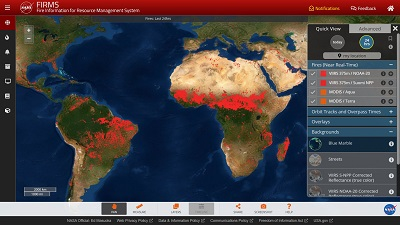
\includegraphics[width=3.21875in,height=\textheight]{fire_index.jpg}}
\href{https://iri.columbia.edu/our-expertise/climate/forecasts/seasonal-climate-forecasts/}{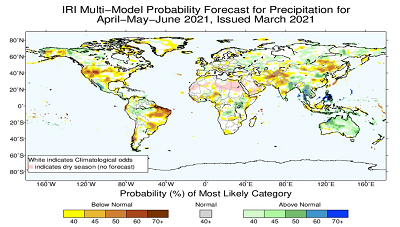
\includegraphics[width=3.16667in,height=\textheight]{Seasonal_Climate Forecast.png}}

Source 1. Fire Data. Source 2. Seasonal CLimate Forecast.

\href{https://iri.columbia.edu/our-expertise/climate/forecasts/seasonal-climate-forecasts/}{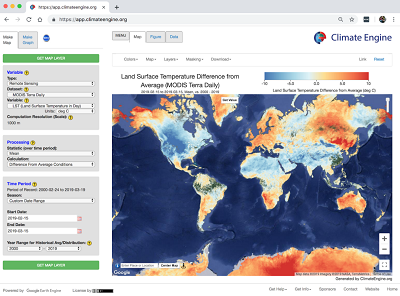
\includegraphics[width=3.11458in,height=\textheight]{climate_engine.png}}
\includegraphics[width=3.02083in,height=\textheight]{https://spatialagent.org/WaterInAgriculture/images/34.jpg}

Source 2. Climate Engine.

\hypertarget{help-feedback}{%
\subsection{Help \& feedback}\label{help-feedback}}

For additional help or to submit feedback or bug reports, please
contact:\\
Didi Adisaputro Climatology Section
\href{mailto:Sect.head.climatology@sinarmas-agri.com}{\nolinkurl{Sect.head.climatology@sinarmas-agri.com}}

\end{document}
